% ============================================================
% FIFA World Cup 2026 — Importation Risk
% InsightNet meeting — 10-minute talk
% ============================================================
\documentclass[aspectratio=169, 11pt]{beamer}

% --- Theme ---------------------------------------------------
\usetheme{Madrid}
\usecolortheme{beaver}
\setbeamertemplate{navigation symbols}{}
\setbeamerfont{frametitle}{size=\large, series=\bfseries}

% --- Packages ------------------------------------------------
\usepackage{amsmath, amssymb}
\usepackage{booktabs}
\usepackage{graphicx}
\usepackage{xcolor}
\usepackage{hyperref}

% --- Colours -------------------------------------------------
\definecolor{wcred}{RGB}{190, 30, 45}
\definecolor{wcblue}{RGB}{0, 64, 140}
\definecolor{wcgray}{RGB}{100, 100, 100}
\definecolor{baseline}{RGB}{149, 165, 166}
\definecolor{wcadj}{RGB}{230, 126, 34}
\definecolor{sched}{RGB}{41, 128, 185}

% --- Metadata ------------------------------------------------
\title[WC 2026 Importation Risk]{%
  Estimating Infectious Disease Importation Risk\\
  during the 2026 FIFA World Cup}
\author{Jose L. Herrera-Diestra}
\institute{Tarleton State University}
\date{June 2026}

% ============================================================
\begin{document}
% ============================================================

% --- 1. Title -----------------------------------------------
\begin{frame}
  \titlepage
\end{frame}

% --- 2. Motivation ------------------------------------------
\begin{frame}{Why does this matter?}
  \begin{columns}[T]
    \begin{column}{0.55\textwidth}
      \footnotesize\textbf{2026 FIFA World Cup — key facts}
      \begin{itemize}\footnotesize
        \item \textbf{48 nations}, largest WC in history
        \item \textbf{11 US host cities}, June 11 -- July 19
        \item $\sim$85 million international visitors projected
              for the US in 2026 (NTTO annual forecast)
        \item Visitors from every qualified nation, many in
              disease-endemic regions
      \end{itemize}
      \begin{center}
        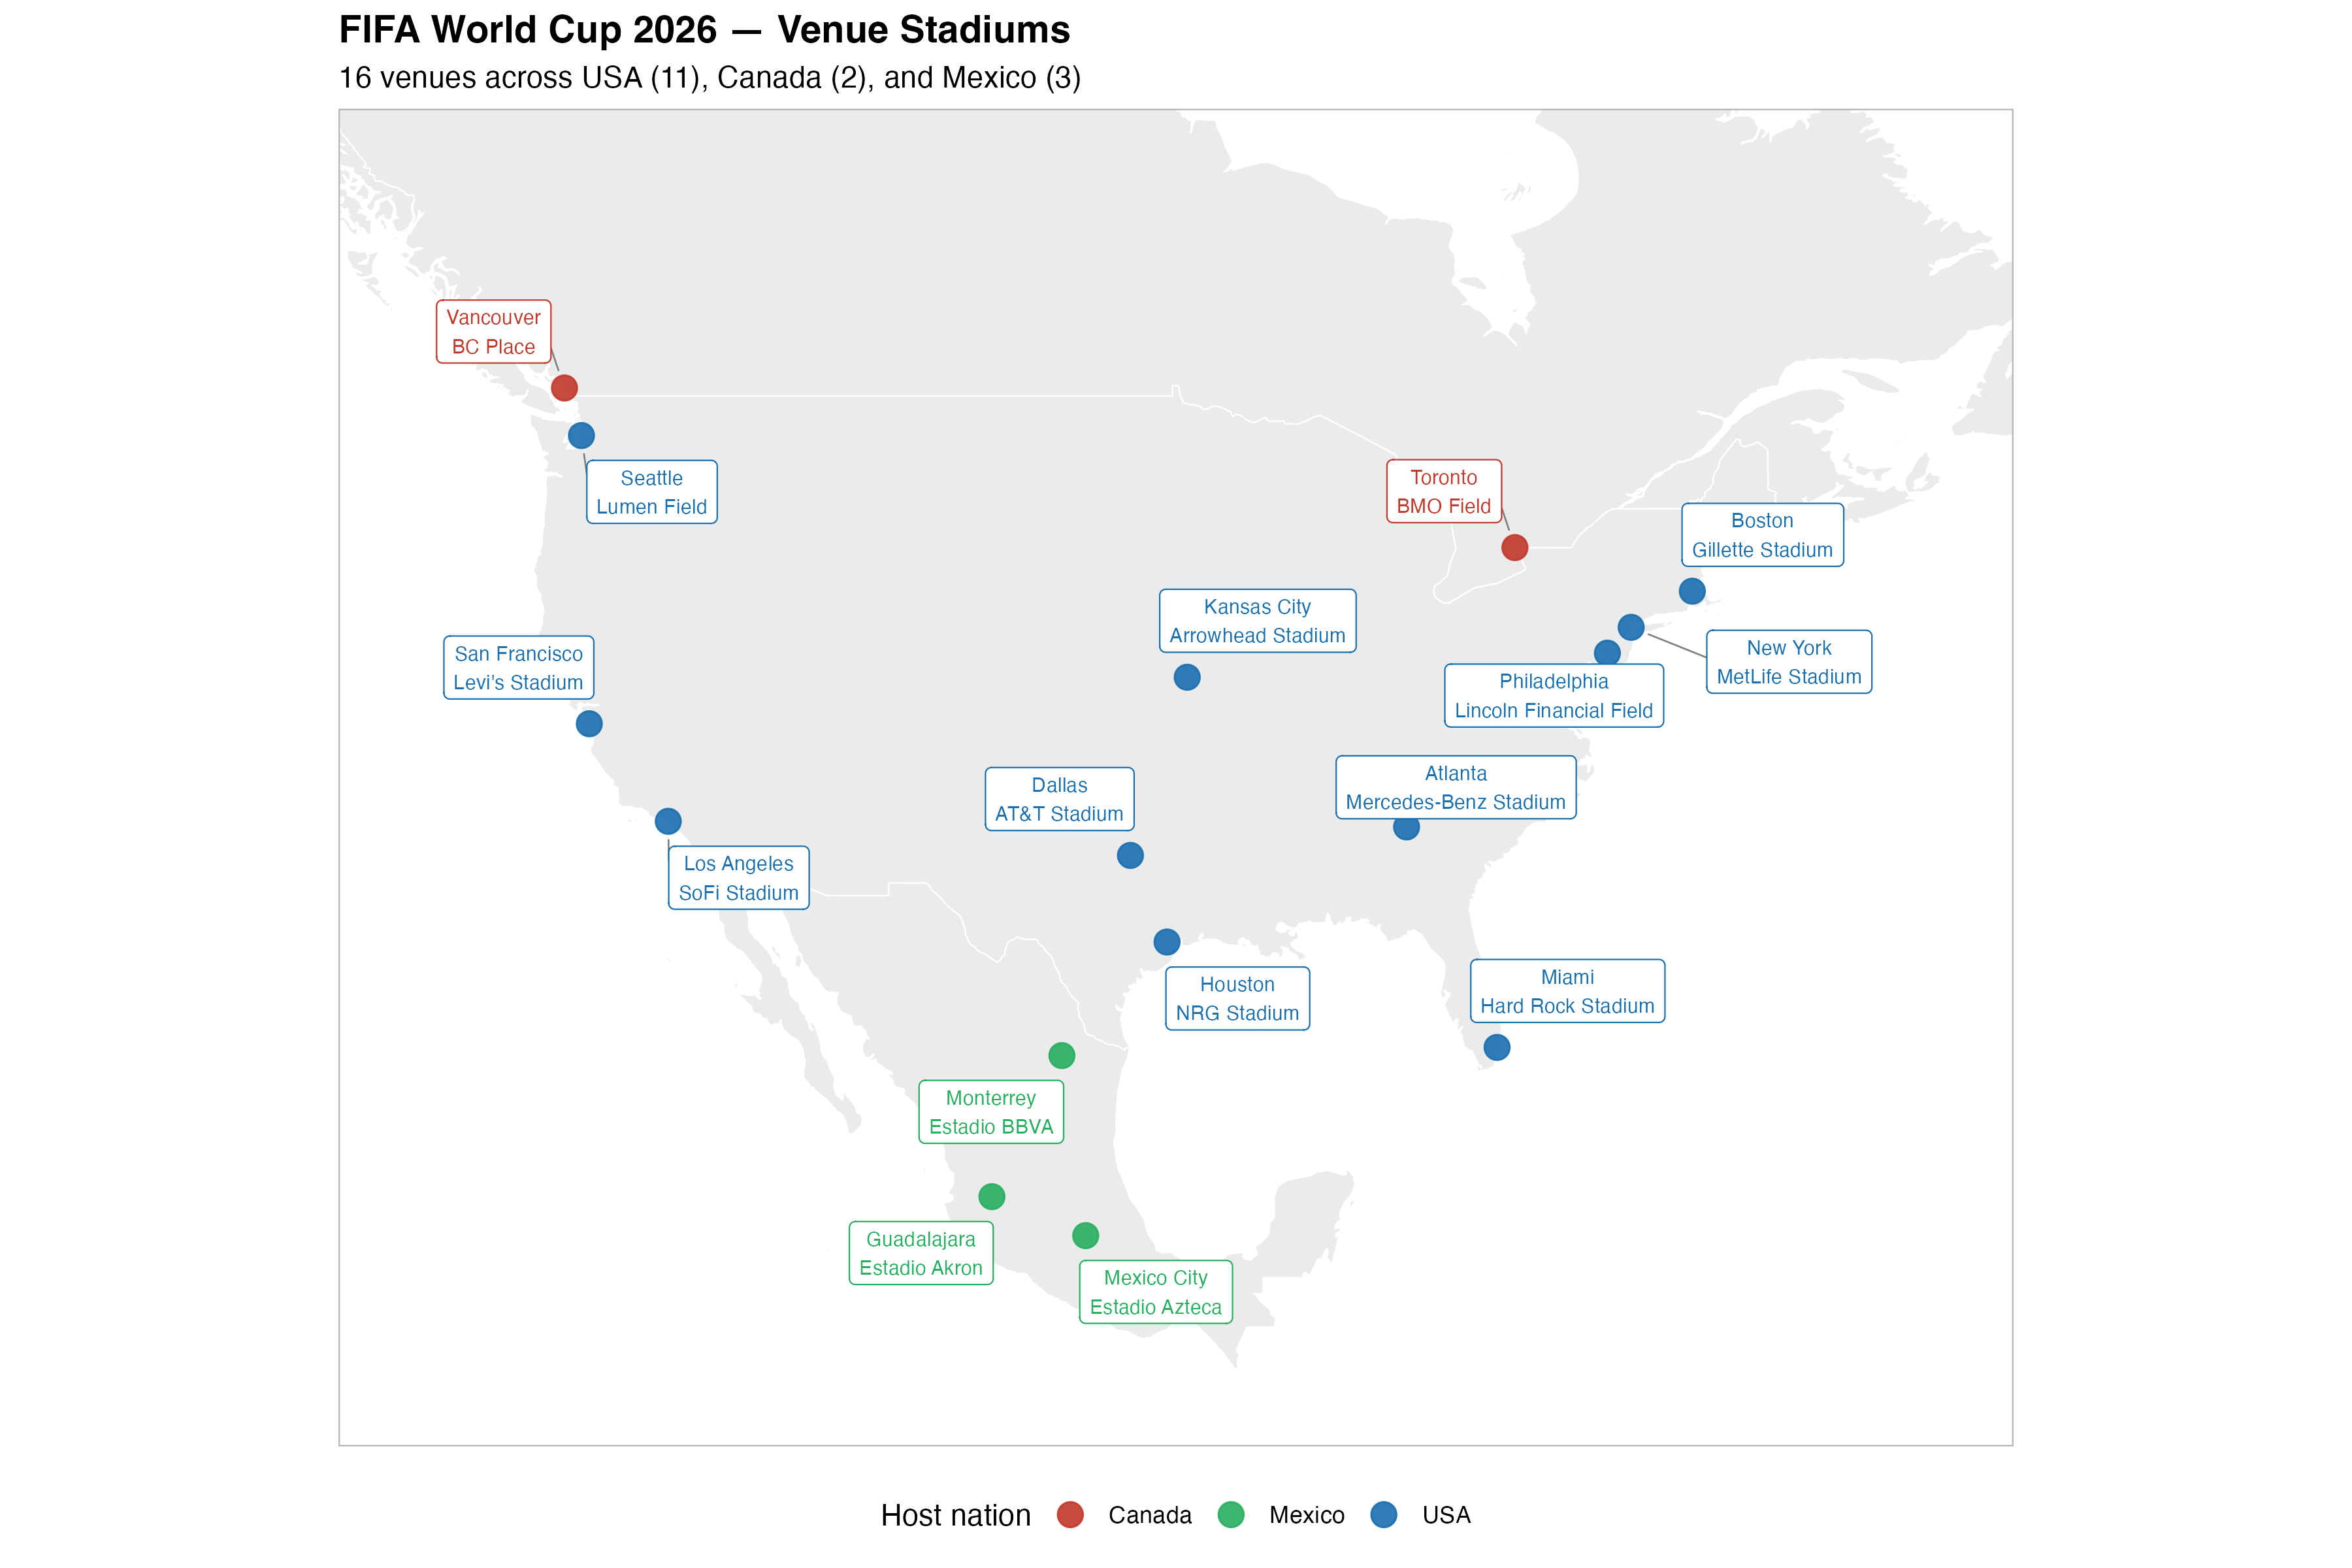
\includegraphics[width=\textwidth, height=0.45\textheight,
          keepaspectratio]{../Figures/wc2026_venue_map.png}
      \end{center}
    \end{column}
    \begin{column}{0.42\textwidth}
      \begin{block}{Research question}
        \footnotesize\textit{What is the probability that dengue,
        influenza, malaria, measles, or pertussis is imported
        into each US host city during June 2026 --- and which
        source countries drive that risk?}
      \end{block}
      \vspace{0.5em}
      \footnotesize\textbf{Goal}: build a quantitative importation
      risk baseline from open surveillance and travel data to help
      prioritize preparedness efforts by venue city.
    \end{column}
  \end{columns}
\end{frame}

% --- 3. Data ------------------------------------------------
\begin{frame}{Data sources}
  \begin{columns}[T]
    \begin{column}{0.48\textwidth}
      \textbf{Travel data}
      \begin{itemize}
        \item \textbf{COR / I-94} (CBP): monthly arrivals by
              country of residence --- June 2024 baseline
        \item \textbf{BTS T-100}: nonstop segment data,
              country-level routing fractions to each US
              venue city (mean June 2023--2025)
        \item \textbf{NTTO 2026 Forecast}: official travel
              projections, 12 top source markets
      \end{itemize}
    \end{column}
    \begin{column}{0.48\textwidth}
      \textbf{Disease surveillance}
      \begin{itemize}
        \item \textbf{Dengue}: WHO Global Dengue Surveillance
              (monthly, Dec 2025)
        \item \textbf{Influenza}: WHO FluNet / GISRS
              (ISO weeks 22--26, 2023--2025)
        \item \textbf{Malaria}: WHO Global Malaria Programme
              (2024 annual)
        \item \textbf{Measles / Pertussis}: WHO Immunization
              Data portal (annual, 2025)
      \end{itemize}
    \end{column}
  \end{columns}
  \vspace{0.5em}
  \begin{block}{}
    \centering\small
    Open-access sources throughout --- straightforward to update
    as new data become available.
  \end{block}
\end{frame}

% --- 4. Framework -------------------------------------------
\begin{frame}{Poisson importation framework}
  \textbf{Core equation} — expected importations of disease $d$
  into city $v$:
  \[
    \Lambda_{v,d}
    = \sum_{c}\,
      \underbrace{N_{c,v}}_{\text{arrivals}}
      \times
      \underbrace{\rho_d \cdot \frac{C_{c,d}}{P_c}}_{\text{per-traveller incidence}}
      \times
      \underbrace{p_d}_{\substack{\text{travel while}\\\text{infectious}}}
    \qquad
    P(X \geq 1) = 1 - e^{-\Lambda_{v,d}}
  \]

  \medskip
  \textbf{Three nested models} for arrivals $N_{c,v}$:
  \begin{center}
  \small
  \begin{tabular}{clll}
    \toprule
    & \textbf{Model} & \textbf{Travel volume} & \textbf{City routing} \\
    \midrule
    M1 & \textcolor{baseline}{\textbf{Baseline}}
       & COR June 2024 & T-100 fractions \\
    M2 & \textcolor{wcadj}{\textbf{WC-adjusted}}
       & 2026 NTTO projections ($\phi_c$) & T-100 fractions \\
    M3 & \textcolor{sched}{\textbf{Schedule-driven}}
       & 2026 + WC fan decomposition & Match schedule \\
    \bottomrule
  \end{tabular}
  \end{center}

  \medskip
  \textbf{Uncertainty}: $\rho_d$ and $p_d$ sampled from
  Uniform literature ranges (5,000 MC draws) $\Rightarrow$
  MC median $+$ 95\% uncertainty interval on every estimate.
\end{frame}

% --- 5. Three models ----------------------------------------
\begin{frame}{Three nested models — what each one adds}
  \begin{columns}[T]

    \begin{column}{0.31\textwidth}
      \begin{block}{\textcolor{baseline}{\textbf{M1 — Baseline}}}
        \scriptsize
        No WC adjustment; routine travel only.\\[4pt]
        \textbf{Growth factor:}
        \[ \phi_c = 1 \quad \forall\, c \]
        \textbf{Arrivals:}
        \[ N_{c,v}^{\text{M1}} = N_{c,24}^{\text{COR}}
           \cdot f_{c,v}^{\text{T100}} \]
        {\tiny $f_{c,v}^{\text{T100}}$: T-100 routing fraction
        (mean Jun 2023--2025)}\\[4pt]
        \textit{Answers}: what does baseline
        importation risk look like without
        any tournament effect?
      \end{block}
    \end{column}

    \begin{column}{0.31\textwidth}
      \begin{block}{\textcolor{wcadj}{\textbf{M2 — WC-adjusted}}}
        \scriptsize
        WC travel surge applied; same routing.\\[4pt]
        \textbf{Growth factor (tiered):}
        \[
          \phi_c = \begin{cases}
            \dfrac{V_{c,26}}{V_{c,24}} & \text{NTTO top-12}\\[4pt]
            1.174 & \text{WC-qualified}\\
            1.077 & \text{non-qualified}
          \end{cases}
        \]
        \textbf{Arrivals:}
        \[ N_{c,v}^{\text{M2}} = N_{c,24}^{\text{COR}}
           \cdot \phi_c \cdot f_{c,v}^{\text{T100}} \]
        \textit{Answers}: how much does the
        WC surge alone amplify risk?
      \end{block}
    \end{column}

    \begin{column}{0.31\textwidth}
      \begin{block}{\textcolor{sched}{\textbf{M3 — Schedule-driven}}}
        \scriptsize
        \setlength{\abovedisplayskip}{2pt}
        \setlength{\belowdisplayskip}{2pt}
        \setlength{\abovedisplayshortskip}{0pt}
        \setlength{\belowdisplayshortskip}{2pt}
        Same $\phi_c$ as M2; fans routed by match schedule.\\[2pt]
        \textbf{Travel decomposition:}
        \[ N_c^{\text{WC}} = N_{c,24}^{\text{COR}}
           \cdot \max\!\bigl(0,\,\phi_c - \phi_{\text{base}}\bigr) \]
        \[ N_c^{\text{bg}} = N_{c,24}^{\text{COR}}
           \cdot \phi_c - N_c^{\text{WC}} \]
        \textbf{Arrivals:}
        \[ N_{c,v}^{\text{M3}} =
           N_c^{\text{WC}} \cdot \omega_{c,v}
           + N_c^{\text{bg}} \cdot f_{c,v}^{\text{T100}} \]
        {\tiny $\omega_{c,v} = g_{c,v}/G_c$: schedule routing fraction}\\[3pt]
        \textit{Answers}: does schedule-based
        fan routing shift which cities
        bear the highest risk?
      \end{block}
    \end{column}

  \end{columns}

  \vspace{0.4em}
  \scriptsize
  \textbf{M1 $\to$ M2}: isolates the WC volume effect ($\phi_c$). \quad
  \textbf{M2 $\to$ M3}: isolates schedule-based fan redistribution. \quad
  \textit{All results shown use M3.}
\end{frame}

% --- 6. Result 1: Heatmap -----------------------------------
\begin{frame}{Result 1 — Importation probability across all venues}
  \begin{center}
    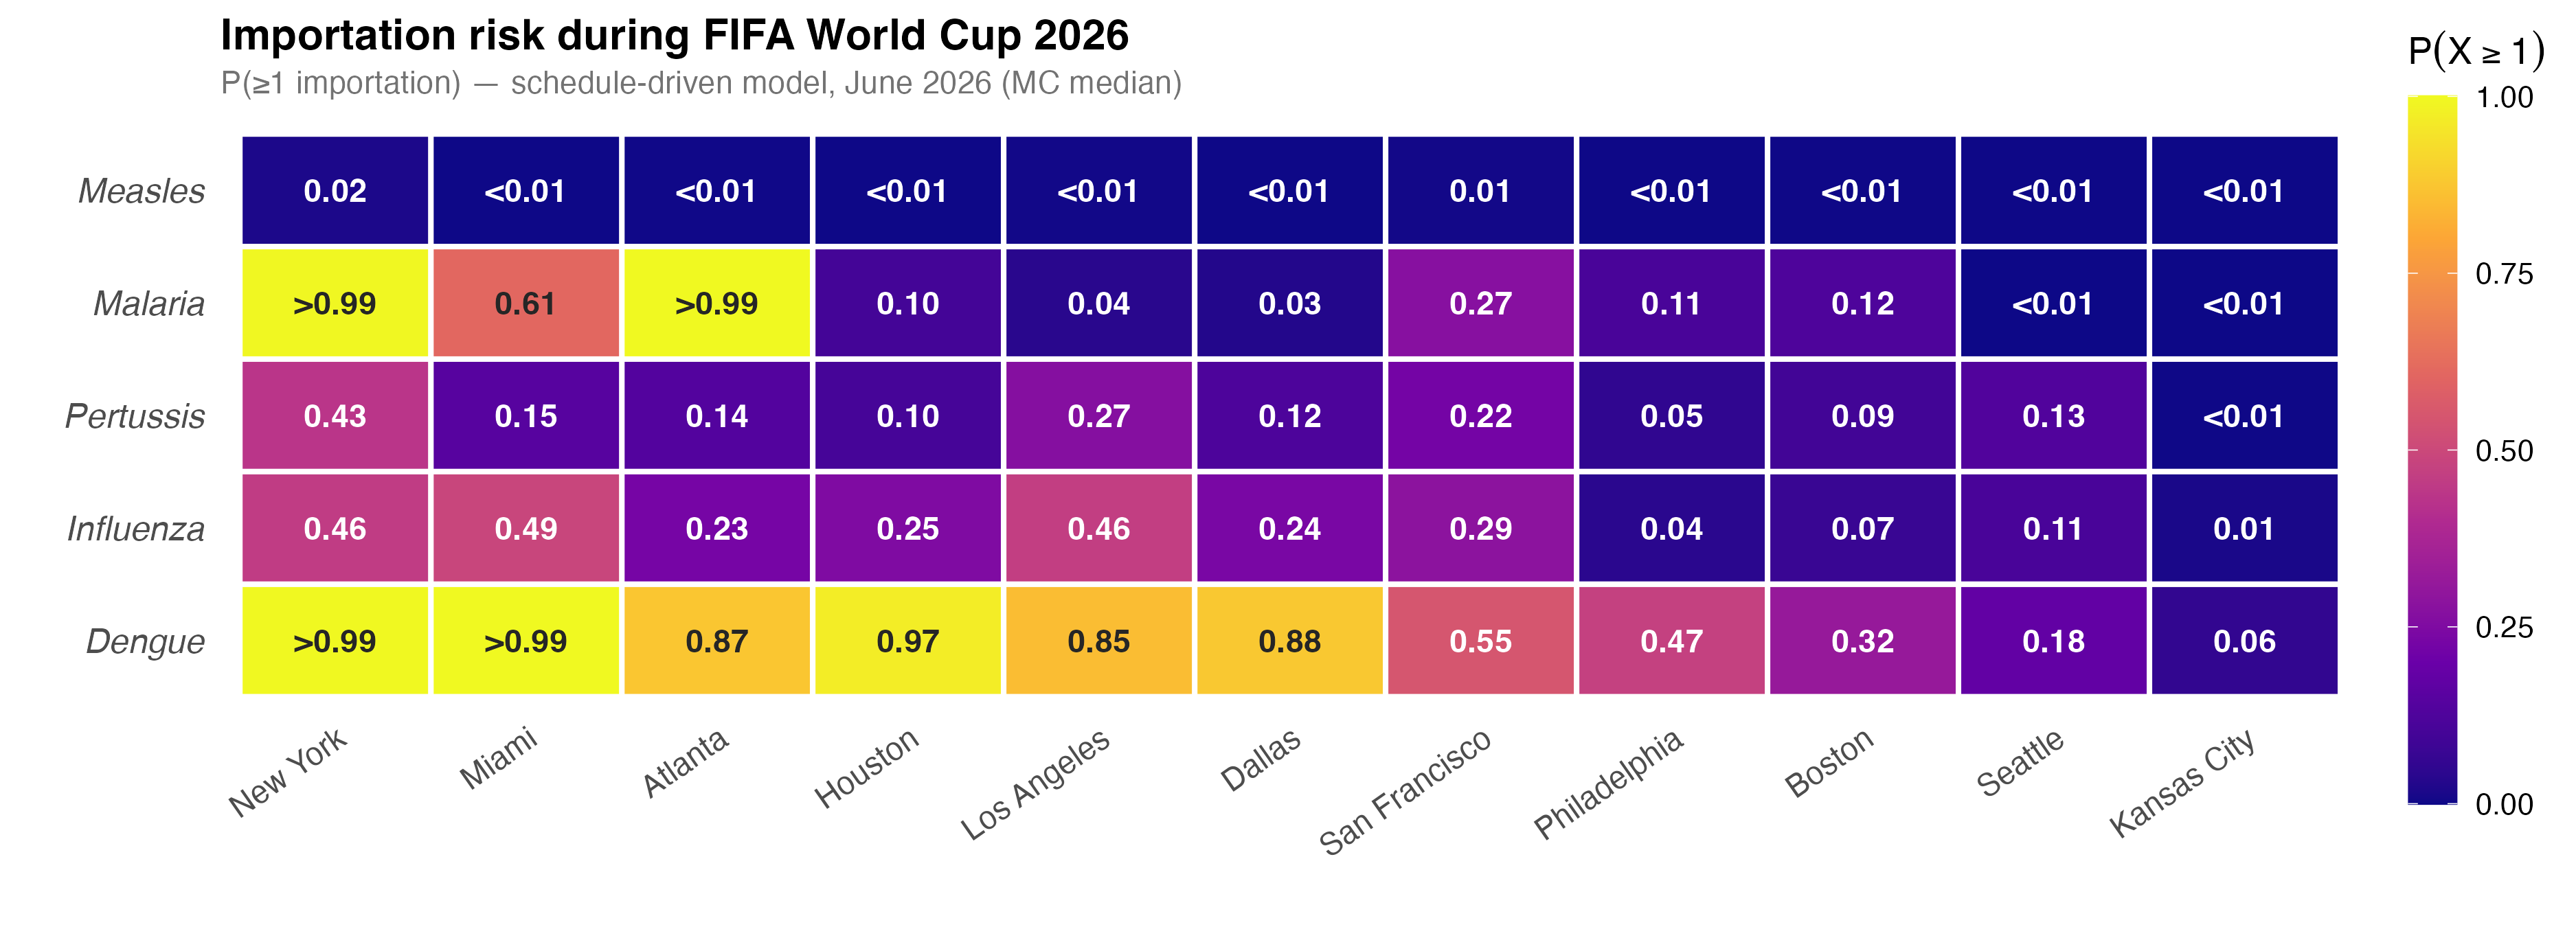
\includegraphics[width=\textwidth, height=0.70\textheight,
      keepaspectratio]{../Figures/fig1_risk_heatmap.png}
  \end{center}
  \vspace{-0.4em}
  {\footnotesize
  $P(\geq 1)$ under the schedule-driven model (MC median, 5,000 draws).
  Dengue leads at most cities ($P>0.99$ at Miami, New York, Houston).
  \textbf{Atlanta exception}: malaria $>$ dengue ($P>0.99$ vs.\ 0.97),
  driven by direct travel from West/Central Africa.
  Measles is consistently lowest.}
\end{frame}

% --- 6. Result 2: Lambda CI ---------------------------------
\begin{frame}{Result 2 — Importation intensity with uncertainty}
  \begin{center}
    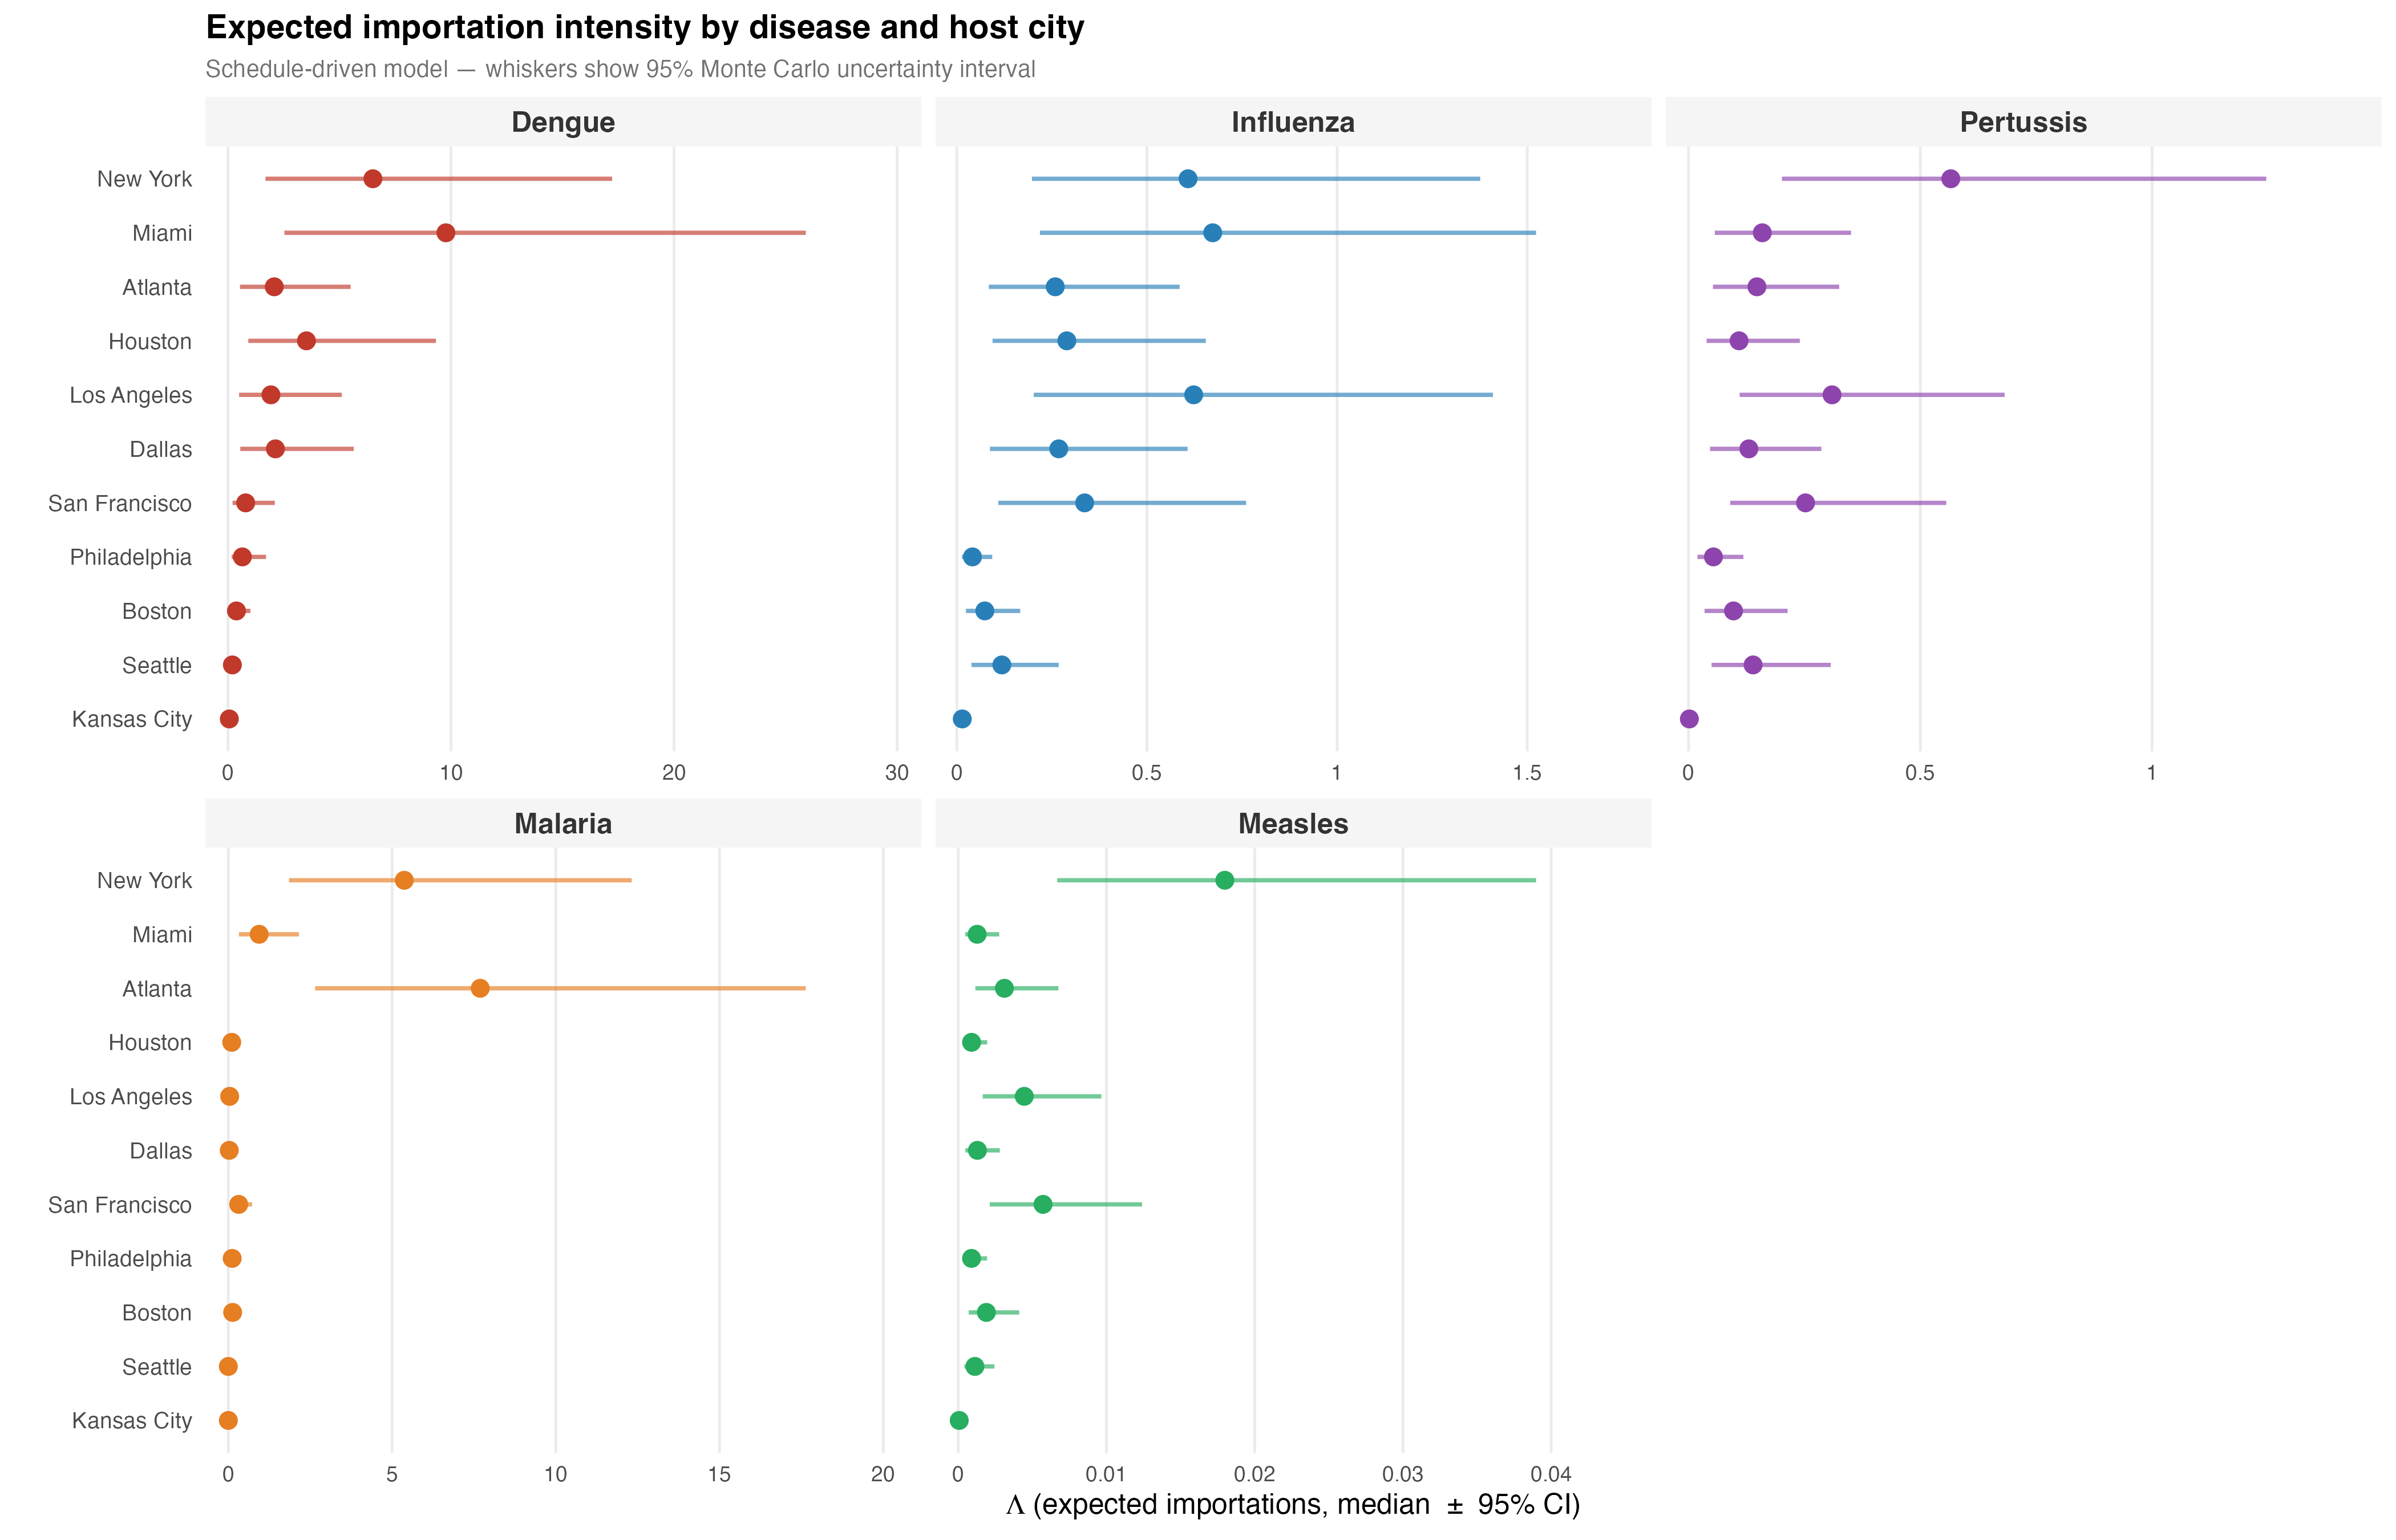
\includegraphics[width=\textwidth, height=0.70\textheight,
      keepaspectratio]{../Figures/fig2_lambda_ci.png}
  \end{center}
  \vspace{-0.4em}
  {\footnotesize
  Bars = MC median $\Lambda$; whiskers = 95\% uncertainty interval.
  Dengue is orders of magnitude above all other diseases.
  Pertussis CIs skew downward (central value is a conservative upper
  bound); dengue and influenza CIs skew upward (may be understated).}
\end{frame}

% --- 7. Result 3: Country drivers ---------------------------
\begin{frame}{Result 3 — Source country drivers}
  \begin{center}
    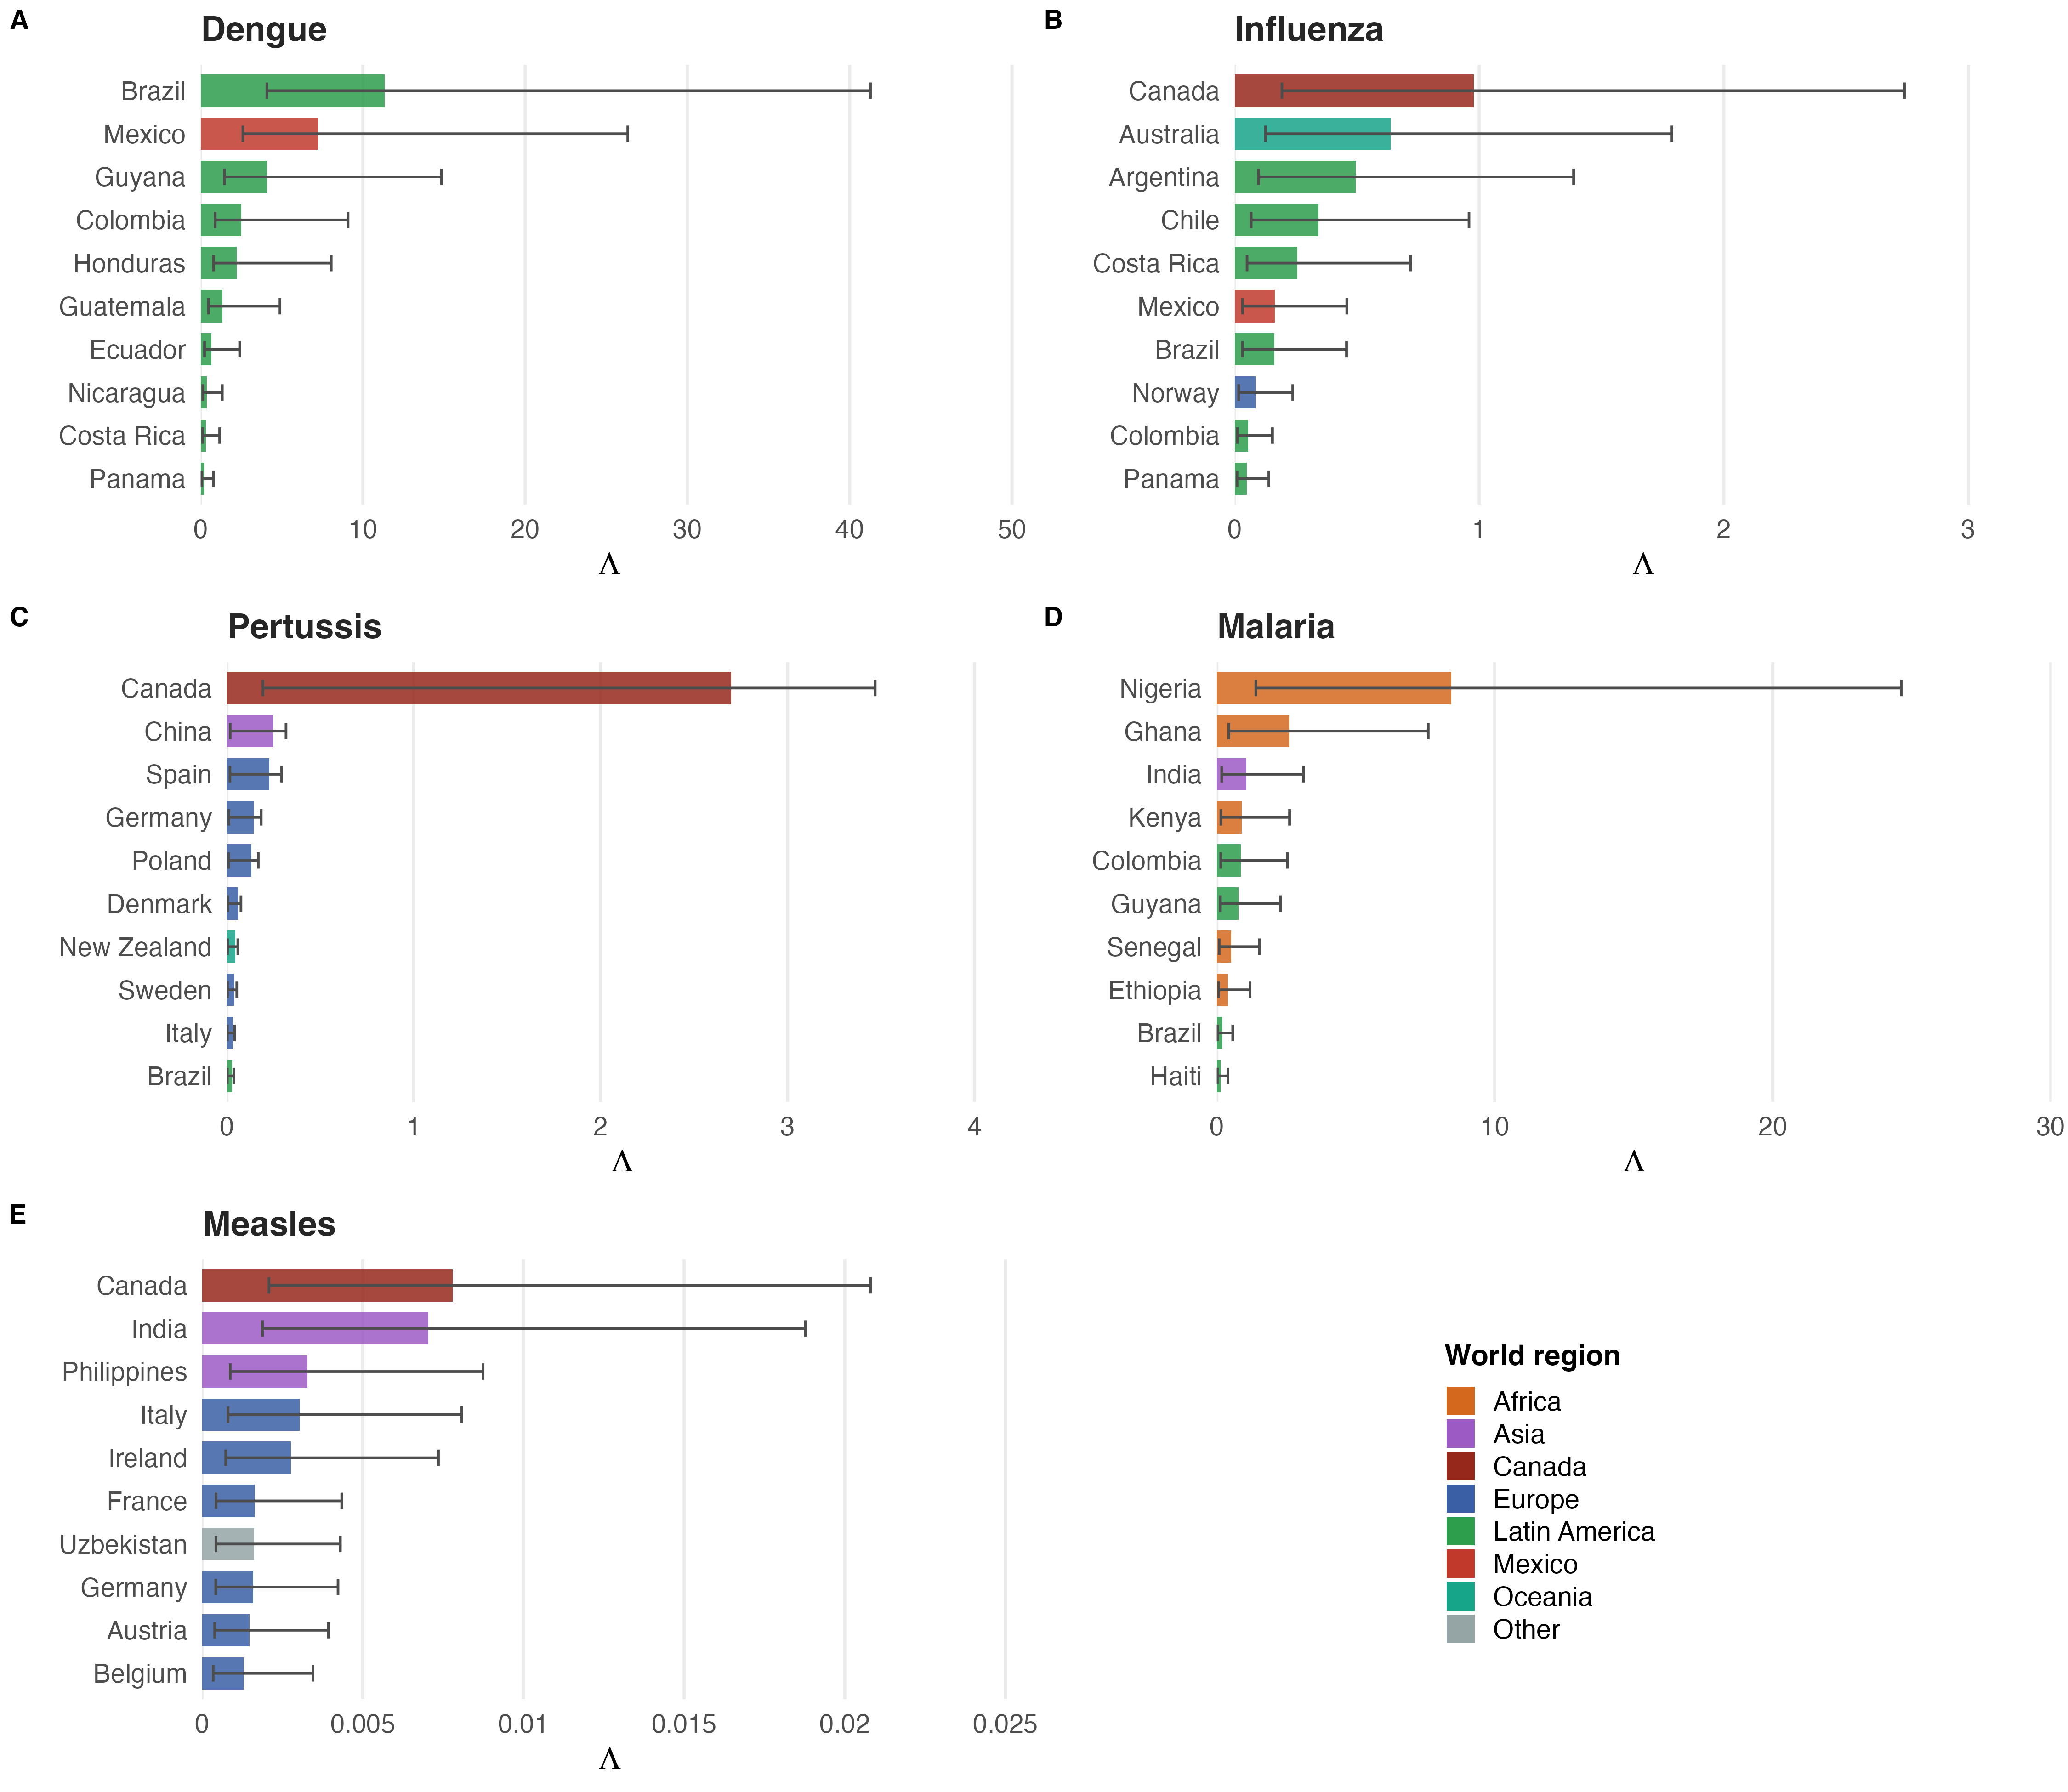
\includegraphics[width=\textwidth, height=0.70\textheight,
      keepaspectratio]{../Figures/fig4_country_drivers.png}
  \end{center}
  \vspace{-0.4em}
  {\footnotesize
  Top 10 source countries per disease (schedule-driven, all 11 US cities).
  Latin America dominates dengue \& influenza; West/Central Africa drives
  malaria; Europe leads pertussis \& measles. Rankings are stable across
  the full MC parameter range.}
\end{frame}

% --- 8. Conclusions -----------------------------------------
\begin{frame}{Conclusions}
  \begin{enumerate}
    \item \textbf{Dengue leads importation risk} at most US venue cities
          ($P(\geq 1)>0.99$ at Miami, New York, Houston) --- robust
          across all parameter assumptions.

    \item \textbf{Atlanta is a notable exception}: malaria probability
          exceeds dengue, driven by direct flights from West and Central
          Africa. City-level heterogeneity matters.

    \item \textbf{Influenza ranks second} at most cities, amplified by
          the Southern Hemisphere winter peak during June.

    \item \textbf{Background tourism dominates}: the WC fan increment
          accounts for only $\approx 8.3\%$ of projected arrivals ---
          pre-existing travel patterns set the baseline risk.

    \item \textbf{The framework is portable and documented}: built
          entirely from publicly available sources, it can be
          deployed for any future mass gathering with minimal lead
          time as travel projections and case data are updated.
  \end{enumerate}

  \vspace{0.3em}
  {\small\textit{A reproducible baseline intended to complement ---
  not replace --- operational intelligence and richer data streams.}}
\end{frame}

% --- 9. Thank you -------------------------------------------
\begin{frame}[plain]
  \vfill
  \begin{center}
    {\Large\textbf{Thank you}}\\[1em]
    \texttt{jherreradiestra@tarleton.edu}\\[0.8em]
    {\small Code \& data:}\\[0.2em]
    {\small\url{https://github.com/jdiestra1977/FIFA_worldCup_2026_risk}}\\[0.6em]
    {\small Preprint:}\\[0.2em]
    {\small\url{https://www.medrxiv.org/content/10.64898/2026.06.03.26354828v1}}
  \end{center}
  \vfill
\end{frame}

% ============================================================
\end{document}
